\section{STFT \& Spectrograms}
\begin{frame}{}
    \LARGE \textbf{STFT \& Spectrograms}
\end{frame}

\begin{frame}[allowframebreaks]{Short-Time Fourier Transform (STFT)}
    \begin{itemize}
        \item STFT is a method to analyze the frequency content of a signal over time.
        \item It involves applying the Fourier Transform to short overlapping segments (frames) of the signal.
        \item The STFT provides a time-frequency representation of the signal.
    \end{itemize}
    \begin{figure}
        \centering
        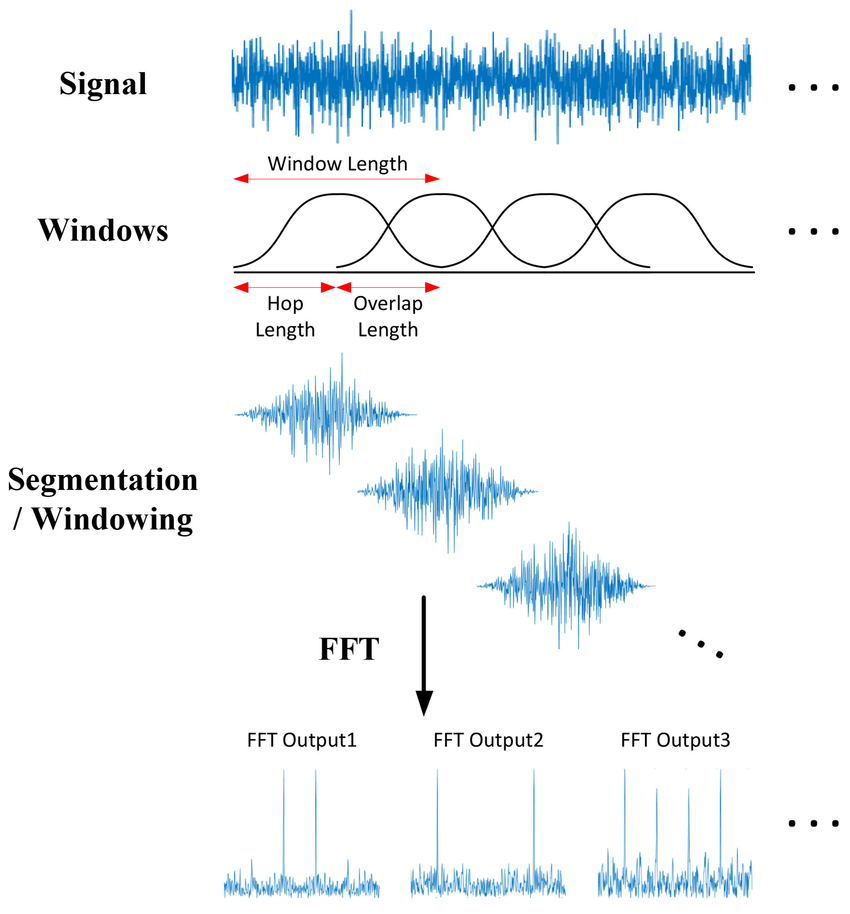
\includegraphics[width=\textwidth,height=0.8\textheight,keepaspectratio]{images/audio-nlp/stft-diagram.png}
        \caption*{STFT process: Signal divided into frames, each transformed into frequency domain.}
    \end{figure}
    \begin{itemize}
        \item The STFT is computed as:
        \[
            STFT(x[n]) = \sum_{m=-\infty}^{\infty} x[m] w[n-m] e^{-j2\pi f m}
        \]
        where $w[n-m]$ is a window function applied to each frame.
    \end{itemize}
\framebreak
    \begin{itemize}
        \item The result is a complex-valued matrix, where each column represents the frequency content of a frame.
        \item The magnitude of the STFT gives the amplitude of each frequency at each time step.
        \item The phase of the STFT provides information about the timing of the frequency components.
    \end{itemize}
    \begin{figure}
        \centering
        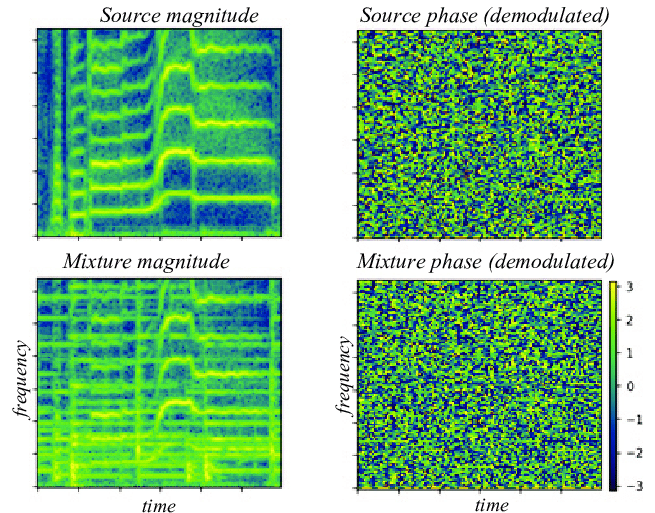
\includegraphics[width=\textwidth,height=0.75\textheight,keepaspectratio]{images/audio-nlp/stft-magnitude-phase.png}
        \caption*{Magnitude and phase of STFT: Magnitude shows amplitude, phase shows timing of frequencies.}
    \end{figure}
\end{frame}

\begin{frame}[allowframebreaks]{Spectrograms}
    \begin{itemize}
        \item A spectrogram is a visual representation of the STFT.
        \item It displays time on the x-axis, frequency on the y-axis, and color intensity represents amplitude.
        \item Spectrograms are widely used in audio analysis, speech recognition, and music processing.
    \end{itemize}
    \begin{figure}
        \centering
        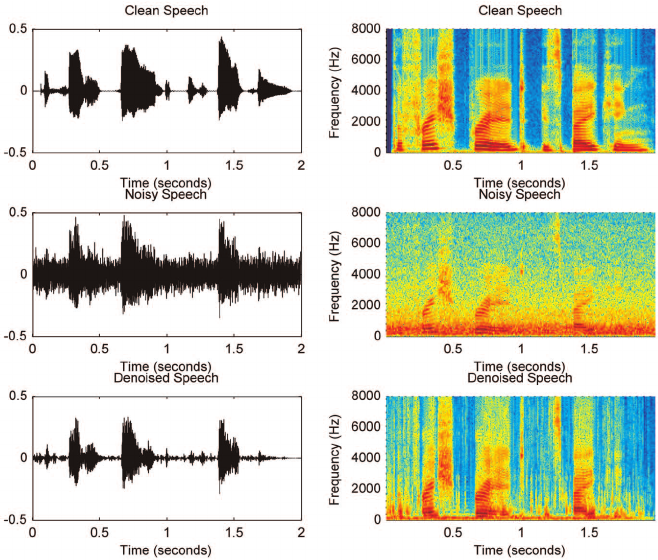
\includegraphics[width=\textwidth,height=0.8\textheight,keepaspectratio]{images/audio-nlp/spectrogram-example.png}
        \caption*{Example of a spectrogram: Time vs Frequency representation of an audio signal.}
    \end{figure}
    \begin{itemize}
        \item Spectrograms can be computed using various window functions (e.g., Hamming, Hanning) and different frame sizes.
        \item They provide insights into how the frequency content of a signal changes over time.
    \end{itemize}
    \begin{figure}
        \centering
        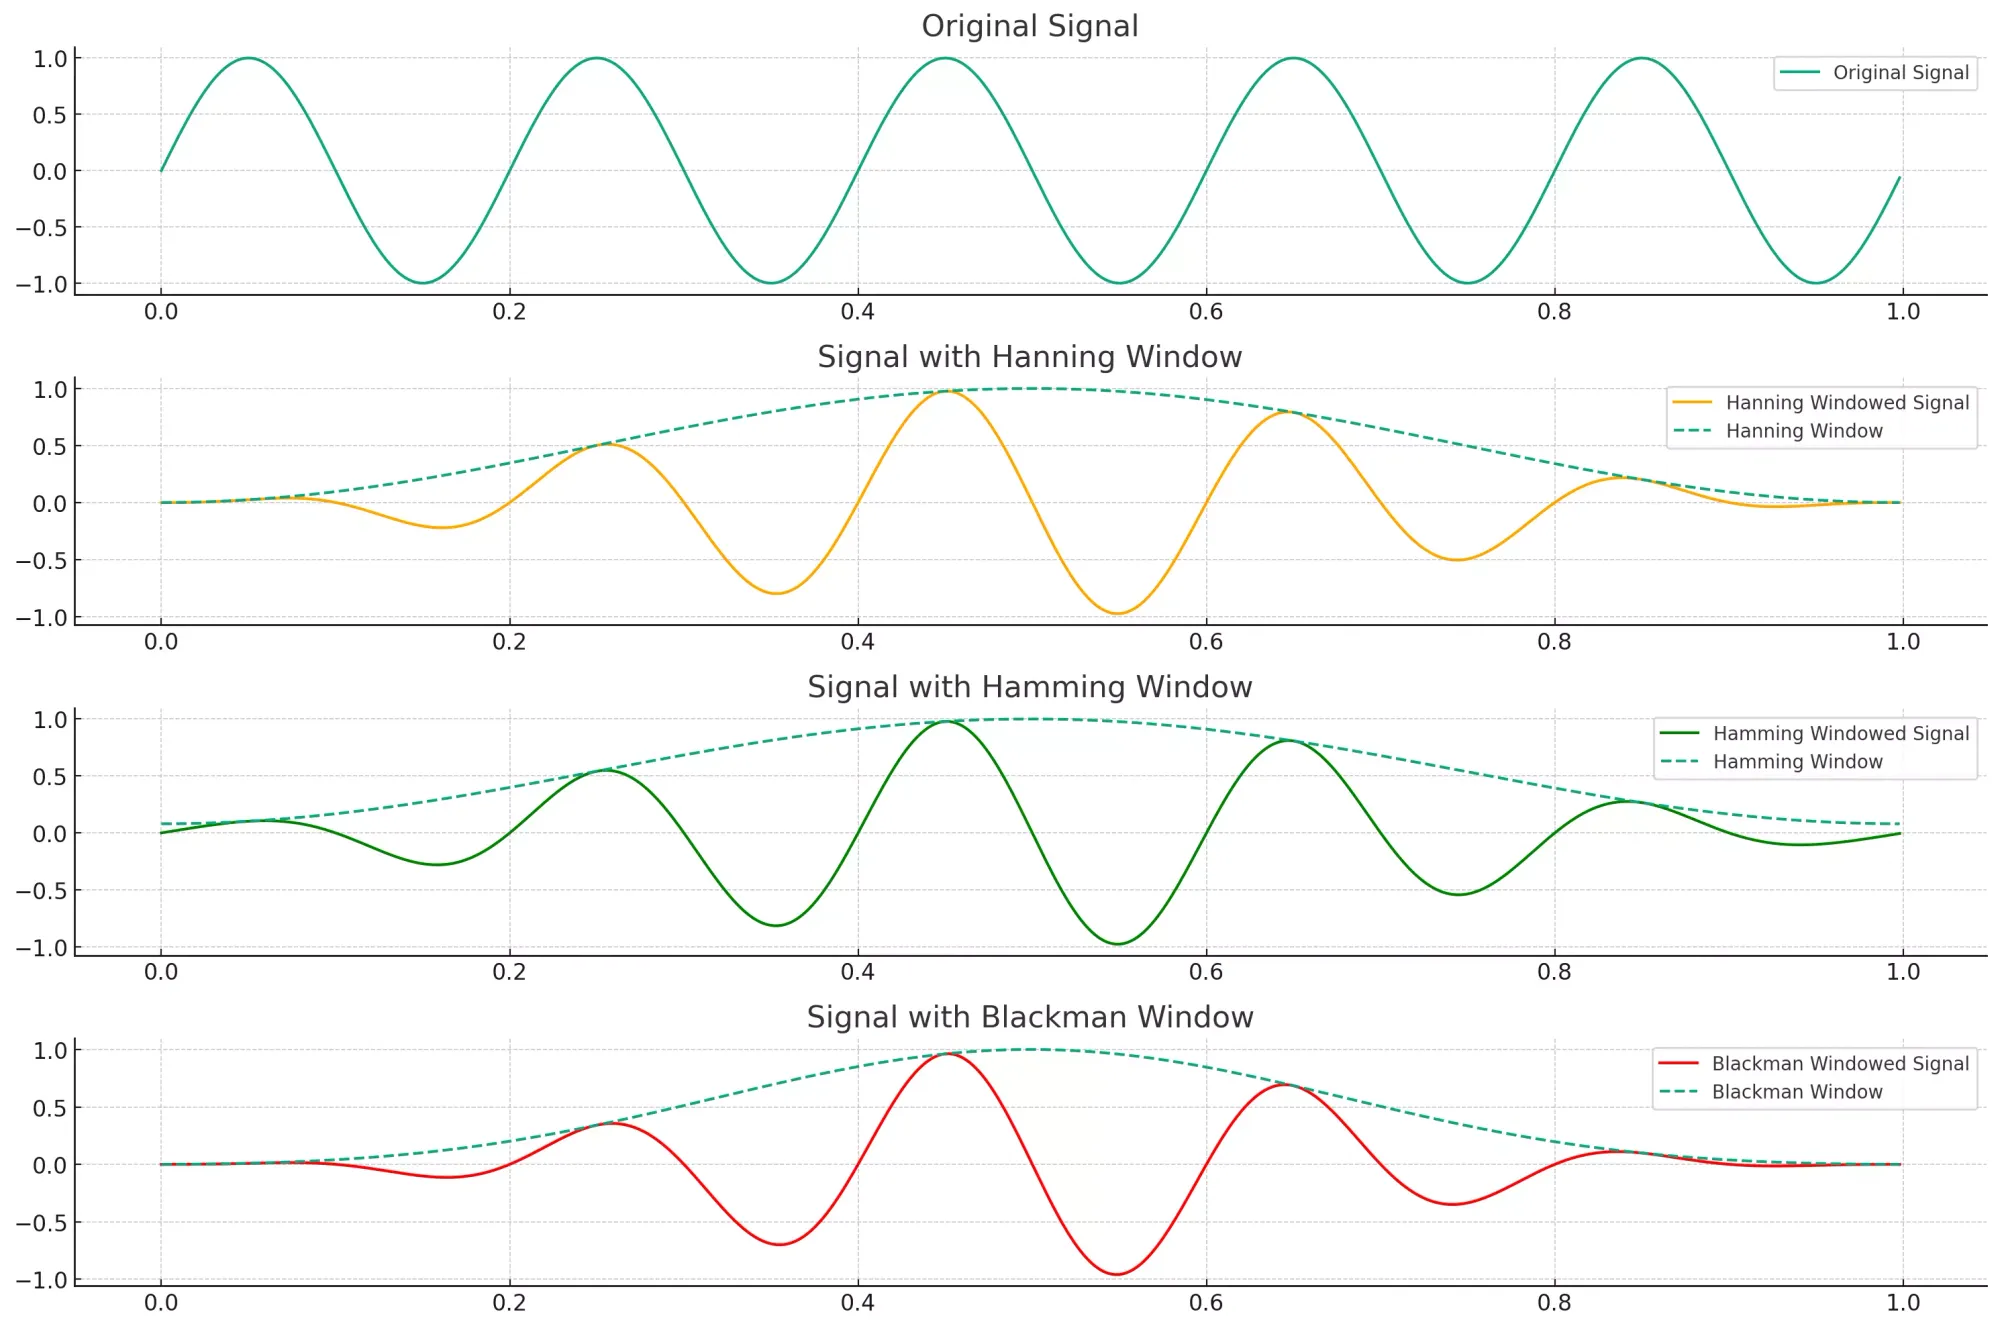
\includegraphics[width=\textwidth,height=0.75\textheight,keepaspectratio]{images/audio-nlp/spectrogram-variations.png}
        \caption*{Spectrogram variations: Different window functions and frame sizes affect the appearance of the spectrogram.}
    \end{figure}
\end{frame}